\documentclass[12pt]{article}
%\usepackage{mathbbold}
\usepackage{ctex}
\usepackage{amsfonts,mathrsfs,amsthm,amssymb,amsmath}
\usepackage{multirow}
\usepackage{bbding}
\usepackage{graphicx,color}
\usepackage{subfig}
\usepackage{rotating}
\usepackage[justification=justified,singlelinecheck=off]{caption}
\captionsetup[table]{name=表格}
\usepackage{bm}
\usepackage{epstopdf}
\usepackage[colorlinks,linkcolor=blue,urlcolor=blue,anchorcolor=blue,citecolor=blue]{hyperref}
\usepackage[noend]{algpseudocode}
\usepackage{algorithmicx,algorithm}
\usepackage{natbib}
\usepackage{longtable,booktabs}
\usepackage{geometry}
\usepackage{CJK}
\usepackage{comment}  % 加载 comment 包
% \usepackage{minted}	  % 代码包
% \usepackage{array}  % 导入 array 宏包
% \usepackage{ragged2e}  % 提供 \RaggedRight
\usepackage{tabularx}  % 导入 tabularx 宏包

%\usepackage{times}
%\usepackage{colortbl}
%\renewcommand{\theequation}{\thesection.\arabic{equation}}%for the form (1.1)(2.8)
\geometry{a4paper, left=2.5cm,right=2.5cm,top=2.5cm,bottom=2.5cm}

\linespread{1.4}

\renewcommand{\tablename}{\footnotesize\textbf{Table}}

%\theoremstyle{plain} \newtheorem{theorem}{Theorem}
%\theoremstyle{definition} \newtheorem{Defi}{Definition}
%\theoremstyle{remark} \newtheorem{Rem}{Remark}
%\theoremstyle{plain} \newtheorem{lemma}{Lemma}

\newtheorem{defi}{\sc Definition}[section]
\newtheorem{theorem}{\sc Theorem}[section]
\newtheorem{lemma}{\sc Lemma}[section]
\newtheorem{prop}{\sc Proposition}[section]
\newtheorem{coro}{\sc Corollary}[section]
\newtheorem{rema}{\sc Remark}[section]
%\newtheorem{exam}{\sc Example}[section]
\renewcommand{\theequation}{{\arabic{section}.\arabic{equation}}}

%the four below to generate roman number
\makeatletter
\newcommand{\rmnum}[1]{\romannumeral #1}
\newcommand{\Rmnum}[1]{\expandafter\@slowromancap\romannumeral #1@}
\newcommand{\M}{\mathcal{M}}
% 报错(Command \I already defined.LaTeX) \newcommand{\I}{\mathcal{I}}
\newcommand{\whb}{\widehat{\bm\beta}}

\makeatother

\renewcommand{\algorithmicrequire}{\textbf{Input:}}
\renewcommand{\algorithmicensure}{\textbf{Output:}}


% 报告主体部分
\begin{document}
\title{羽毛球球员表现的贝叶斯分析:\\ 多重因素下的胜率}		% TODO 使用贝叶斯推理分析和预测体育比赛结果
\date{}

% TODO
\author{shenyuchen$^1$		\\		XXXX大学 XXXX学院}		% \\ 转义+换行
\maketitle

% 摘要
\begin{abstract}
	摘要摘要摘要摘要

\end{abstract}

% TODO - 关键词?摘要
\textbf{关键词}: 贝叶斯;羽毛球;国际羽毛球联合会


\section{引言(Introduction)}
\subsection{贝叶斯发展的三个阶段}
贝叶斯起源于18世纪,一个贝叶斯完整的形成简述成以下三个阶段:

①贝叶斯的发现 \\
由托马斯·贝叶斯(Thomas Bayes)撰写的论文《An Essay towards solving a Problem in the Doctrine of Chances》(《解决机会论问题的论文》)中,首次阐述了这一理论。在本篇论文中,贝叶斯提出通过观察新的样本数据,重新调整对某个事件的发生概率的估计。本篇论文发表于1763年,是在贝叶斯离世后的2年后,由他的朋友理查德·普赖斯(Richard Price)整理并发表出来,让世人才有机会揭开当今在人工智能领域如火如荼的真面目。

②贝叶斯定理的核心思想 \\
如何根据先验知识(已知的数据)调整概率的预测,其数学形式如下:
\begin{equation}
	P(A|B){P(B)}={P(B|A)P(A)}
	\end{equation}
\begin{equation}
    P(A|B)=\frac{P(B|A)P(A)}{P(B)}
\end{equation}

其中:
\begin{itemize}
	\item $P(A|B)$ 是在事件 B 条件给定的情况下,事件 A 发生的概率。
	\item $P(B|A)$ 刚好与 $P(A|B)$ 相反,是在事件 A 条件给定的情况下,事件 B 发生的概率。
	\item $P(A)$、$P(B)$ 分别是事件 A 和事件 B 各自独立发生的概率。
	\end{itemize}

通过贝叶斯定理,可以将先验概率(对事件 A 的初步概率猜测)的基础之上,加上新的证据(新的样本、新的数据)相结合,得到更新后的概率(后验概率)。

③贝叶斯的发展 \\
起初只是停留在理论层面的发展,随着计算机技术的不断发展,尤其是从20世纪以来,贝叶斯方法已经成为现代统计学、人工智能、机器学习中的核心一环。


\subsection{研究背景}
\begin{comment}
	简要介绍羽毛球比赛的相关背景,为什么选择使用贝叶斯推理进行分析。
	\end{comment}

\begin{figure}[h]
	\centering
	\subfloat[中国的踢毽子]{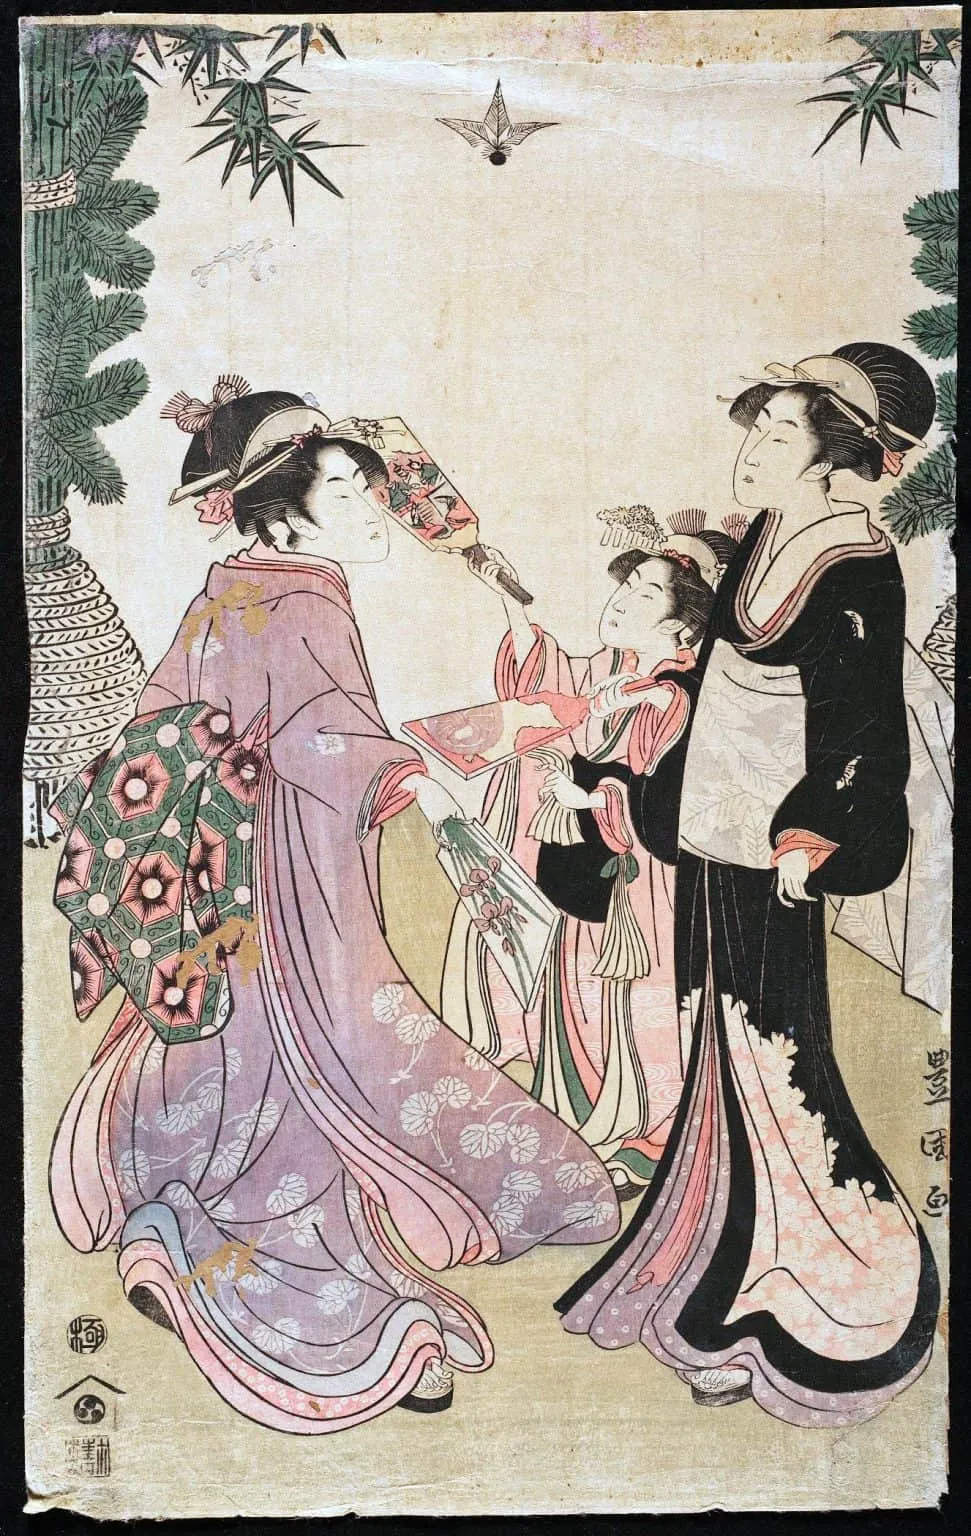
\includegraphics[width=0.48 \linewidth]{../images/history_2_ti_jian_zi}}
	\subfloat[国外打羽毛球的起源]{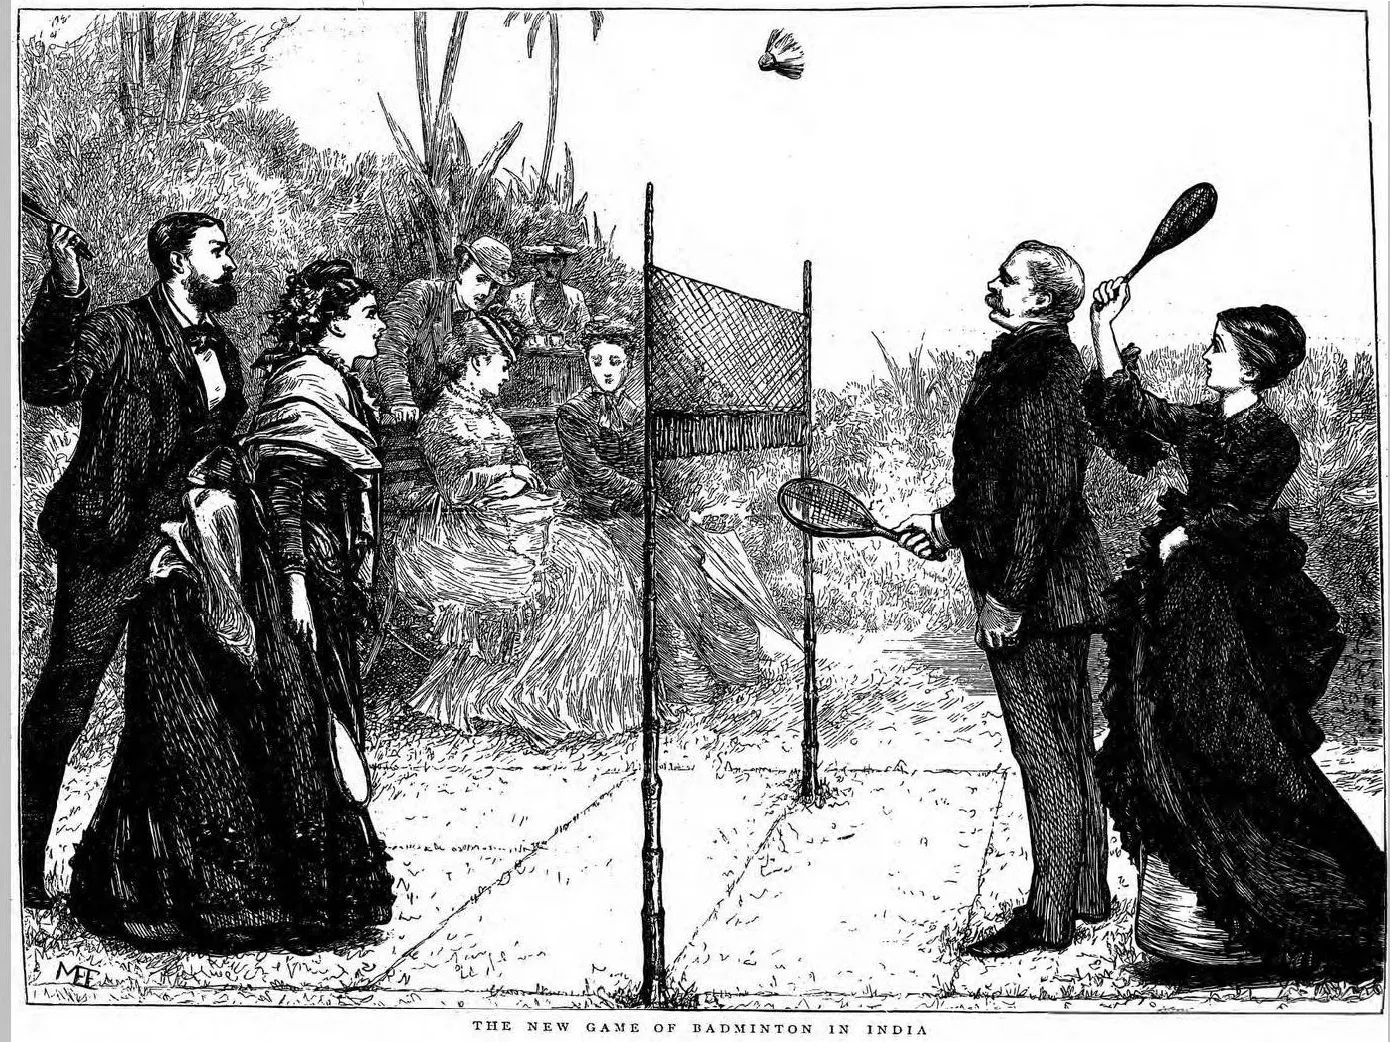
\includegraphics[width=0.48 \linewidth]{../images/history_1}}
	\caption{羽毛球的发展历史}
	\label{fig:histoy}
	\end{figure}


随着体育事业的不断发展,羽毛球的体育赛事逐渐进入人们的视野。
在中国,早在 2000 年前就有人玩一种叫做“踢毽子”的游戏。这个游戏通过用脚相互踢毽子,不仅是一种娱乐活动,还能锻炼人体的灵活性和协调性。(如图 $\ref{fig:histoy}$ 所示)

1877年,英国巴斯羽毛球俱乐部(Bath Badminton Club)在英国巴斯(Bath)首次制定了羽毛球的标准规则,这些规则包括场地尺寸、网高、比赛礼仪和打法等,为羽毛球运动提供了标准和依据,成为现代羽毛球的正式起源。
1893年,由英格兰羽毛球协会(Badminton Association of England)发布,并成为现代羽毛球运动的基础。
1934年,国际羽毛球联合会成立,当时称为 International Badminton Federation(IBF)。
1992年,在巴塞罗那夏季奥运会,羽毛球首次成为正式的奥运项目。
2006年,IBF 更名为羽毛球世界联合会 World Badminton Championships(BWF)。BWF 的总部在马来西亚吉隆坡,目前的成员国已经超过200+个国家。


\subsection{研究目标}
阐述你希望通过贝叶斯推理预测比赛结果,探索相关因素。


\section{数据收集与预处理(Data Collection and Preprocessing)}
\subsection{数据来源}
Badminton World Federation \href{https://bwfbadminton.com/zh-cn/}{羽毛球世界联合会} 简称BWF,是羽毛球运动的全球管理机构,负责组织和管理国际羽毛球赛事,包括世界羽毛球锦标赛和世界羽毛球巡回赛等,提供关于羽毛球比赛的最新动态、赛事结果、运动员信息以及相关技术分析等内容。


\subsection{预处理数据}
TODO
python 爬虫(chatgpt) + 清洗数据
详细描述数据的特征及其重要性。


\section{贝叶斯推理模型(Bayesian Inference Model)}

\subsection{模型概述}
\begin{comment}
	解释贝叶斯定理和你如何应用它进行比赛结果预测。
	详细描述模型的构建过程,包括先验概率、似然函数和后验概率的计算。
	\end{comment}

对于羽毛球球员在多重因素下的胜率这个问题下,我们的任务就是:使用已有的比赛的数据(比如主赛事总得分、对局轮次、最大连续得分、赛点次数、胜负情况、等等)来预测该运动员在未来比赛中的胜利概率。
贝叶斯推理可以帮助我们通过已有的比赛数据(样本数据)来更新模型参数的后验分布,从而做出预测。在本文中,我们将采用 MCMC 方法生成参数的样本,近似计算后验分布,进而计算运动员的胜利概率。

\subsection{贝叶斯推理模型框架}
根据羽毛球世界联合会的官网我们可以获取运动员相关的比赛数据,我们可以使用一个简单的二项分布来描述每场比赛的结果(胜利或者失败),根据贝叶斯定理来更新模型参数的后验分布:

\begin{equation}P(\theta|X)=\frac{P(X|\theta)P(\theta)}{P(X)}\end{equation}

其中:
\begin{itemize}
	\item $P(\theta|X)$ 是后验概率(给定数据 X,参数 $\theta$ 的概率分布)。
	\item $P(X|\theta)$ 是似然函数(给定参数 $\theta$,数据 X 的概率分布)。
	\item $P(\theta)$ 是先验概率(参数 $\theta$ 的先验分布)。
	\item $P(X)$ 是边际似然,通常作为归一化常数。
	\end{itemize}
在比赛预测中,假设每一个比赛的胜负由一个伯努利分布模型来描述:
\begin{equation}
	P(\mathrm{victory}=1|\theta)=\sigma(\theta)
	\end{equation}

其中 $\sigma(\theta)$ 是一个激活函数(比如:sigmoid)将参数 $\theta$ 映射到 [0,1] 范围,表示胜利的概率。

\begin{equation}
	\sigma(x)=\frac{1}{1+e^{-x}}
\end{equation}


\subsection{模型构建}
使用的数据包括如下五个部分:
\begin{itemize}
	\item 主赛事总得分 (\text{total\_scores}):主赛事总得分    运动员在本场主赛事中的总比分。注意每一场不一定是在21分时结束,可能出现延长比赛的情况,同时,也可能发生对手或本人因伤病或其他原因弃赛的情况,这些都将影响最终的总比分。注意,延长赛:如果一局比赛的比分进入到21分之后,两位选手或队伍的得分相差不到两分(例如20-20),这时比赛会进入加赛,直到一方领先2分为止。这种加赛通常没有上限,直到有一方完成领先。
	\item 对局轮次 (\text{rounds\_number}):一般是三局两胜制,也不排除五局三胜,每场主赛事的规则由活动方规定。
	\item 最大连续得分 (\text{max\_consecutive\_points}):与不同运动员对赛时的单次对局时的最大连续得分的数据。
	\item 赛点次数 (\text{game\_points}):羽毛球中的“赛点”指的是比赛中一方可以赢得比赛的关键时刻,即如果该方赢得当前的分数,便会最终获胜。赛点次数是与不同运动员对赛时的单次对局时的赛点次数。
	\item 胜负情况 (\text{victory\_labels}):与不同运动员对赛时的单次对局时的胜负情况。
\end{itemize}

假设我们将这些特征整合成一个向量 x,然后使用逻辑回归模型来预测胜负:
\begin{equation}
    P(\mathrm{victory}=1|\mathbf{x},\theta)=\sigma(\mathbf{x}^T\theta)
\end{equation}
其中,$\theta$ 是逻辑回归模型的参数。

以最新的2024年第47周的\href{https://bwfbadminton.com/zh-cn/player/57945/shi-yu-qi/}{“LI-NING China Masters 2024”}官方数据为例,可整理得以下表格数据:
\begin{table}[h!]
	\centering
	\begin{tabularx}{\textwidth}{|l|X|X|X|X|X|}
	\hline
	\textbf{Opponent} & \textbf{Total Scores} & \textbf{Rounds Number} & \textbf{Max Consecutive Points} & \textbf{Game Points} & \textbf{Victory Labels} \\
	\hline
	Jonatan CHRISTIE & 33 & 2 & 4 & 0 & 0 \\
	Kunlavut VITIDSARN & 42 & 2 & 6 & 4 & 1 \\
	Chico Aura DWI WARDOYO & 42 & 2 & 7 & 3 & 1 \\
	Chia Hao LEE & 42 & 2 & 7 & 5 & 1 \\
	\hline
	\end{tabularx}
	\caption{LI-NING China Masters 2024 Results}
\end{table}

\subsection{马尔可夫链蒙特卡罗(MCMC)方法}
马尔可夫链蒙特卡罗(MCMC)是一种通过构造一个马尔可夫链来模拟目标分布的抽样方法。MCMC 方法可以应用于任何贝叶斯模型,特别是当模型较复杂,无法直接计算后验概率时。MCMC 可以帮助我们通过采样来近似后验分布,我们使用 Metropolis-Hastings 算法来生成后验分布的样本。算法步骤如下:
\begin{enumerate}
	\item 选择初始参数 $\theta^{(0)}$ 。
	\item 通过跳跃选择新的参数 $\theta^{\prime}$ 。
	\item 计算接受概率 $\alpha(\theta,\theta^{\prime})$,并决定是否接受 $\theta^{\prime}$:
	\begin{equation}
		\alpha(\theta,\theta^{\prime})=\min\left(1,\frac{P(D|\theta^{\prime})P(\theta^{\prime})}{P(D|\theta)P(\theta)}\right)
	\end{equation}
	\item 如果接受 $\theta^{\prime}$,则 $\theta^{(t+1)}=\theta^{\prime}$,否则保持 $\theta^{(t+1)}=\theta^{(t)}$ 。
	\item 重复以上过程,直到收敛。
\end{enumerate}


\section{实验与结果(Experiment and Results)}
介绍如何进行模型训练、验证和评估。

展示模型的预测准确性、评估指标(如准确率、精度、召回率等)。

TODO 代码说明和效果展示
data.m
bayesian\_predictive\_model.m


\section{讨论(Discussion)}
分析模型的优缺点,以及可能影响预测结果的因素(如球员状态、比赛场地等)。

\
讨论结果的实际意义以及如何改进模型。


\section{结论(Conclusion)}
总结研究结果,提出未来研究方向。
模型改进:可以尝试加入更多的特征,如比赛场地、球员的身体状况等,改进模型的预测效果。

\
其他机器学习方法:除了贝叶斯推理,还可以尝试使用其他机器学习方法(如决策树、随机森林等)进行对比分析。






% 参考文献
\begin{comment}
	A mathematical analysis of badminton scoring systems

	羽毛球的历史介绍:https://stringsandpaddles.com/the-history-of-badminton/
\end{comment}
\begin{thebibliography}{100}
	\expandafter\ifx\csname natexlab\endcsname\relax\def\natexlab#1{#1}\fi
	\expandafter\ifx\csname url\endcsname\relax
	\def\url#1{\texttt{#1}}\fi
	\expandafter\ifx\csname urlprefix\endcsname\relax\def\urlprefix{URL }\fi

\bibitem[{Battey et al.(2018)}]{battey2018distributed} 
Battey, H., Fan, J., Liu, H., Lu, J. and Zhu, Z., 2018. Distributed testing and estimation under sparse high dimensional models. \textit{Annals of statistics}, \textbf{46}, 1352–1382.

\bibitem[Chang et al.(2017)]{chang2017divide}
Chang, X., Lin, S.B. and Wang, Y., 2017. Divide and conquer local average regression. \textit{Electronic Journal of Statistics}, \textbf{11}, 1326-1350.

\end{thebibliography}


\end{document}


